\recipe{Dom and Dee’s Cardamom Buns}
\label{recipe:cardamom_buns}
\makes{many}
\totaltime{A good while}
\source{Dom}


\begin{ingredients}

  \item 35 cardamom pods
  \item 350ml full-fat milk
  \item 200g butter (cubed)
  \item 500g strong white bread flour
  \item 225g caster sugar
  \item 7g sachet dried yeast
  \item \qty{0.5}{\teaspoon} ground cinnamon
  \item Vegetable oil
  \item 1 large egg
  \item \qty{0.5}{\teaspoon} salt
\end{ingredients}

\begin{figure}[h]
  	\centering
  	
  	\begin{tikzpicture}
  		% Save the image in a box to get its dimensions
  		\sbox0{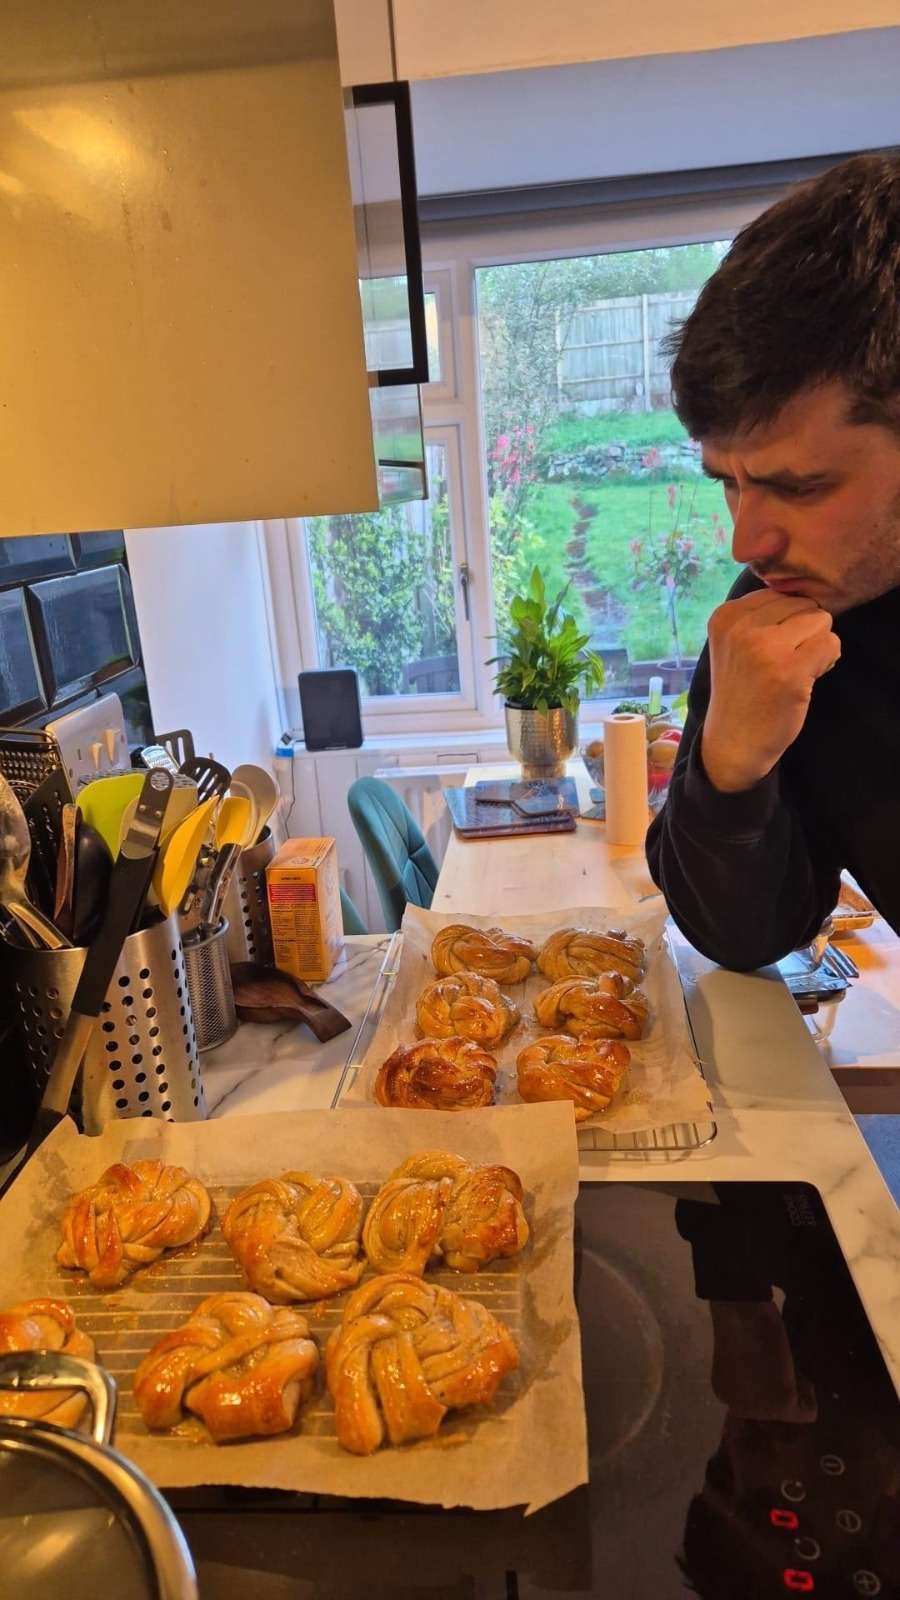
\includegraphics[width = 0.5\linewidth]{images/domCardamonBuns.jpeg}}%
  
  		% Draw a clipping rectangle with rounded corners
  		\path[clip, rounded corners=0.5cm] (0,0) rectangle (\wd0,9cm);
  
  		% Place the image inside the clipped area
  		\node[inner sep=0pt, outer sep=0pt, anchor=south west] at (0, -2) {\usebox0};
	\end{tikzpicture}

\end{figure}

\begin{method}
  	Crack open 10 of the cardamom pods with a pestle and mortar, and tip into a saucepan. Add the milk
and warm until steaming but not boiling. Add 50g butter (leave the remaining butter at room
temperature to soften) and set aside to cool until lukewarm, swirling the pan from time to time to
encourage the butter to melt.

Put the flour, 75g of the sugar, the yeast, cinnamon and 1/2 tsp salt into a large bowl. Mix until well
combined. When the milk has cooled, strain it through a sieve into the flour, discarding the cardamom.
Using a wooden spoon mix to form a soft dough. Tip onto a work surface and knead for 10 mins, until
the dough is smooth and stretchy. Clean the bowl, lightly grease with oil, then return the dough to the
bowl and turn it over until well coated in oil. Cover the bowl with a tea towel or cling film and leave to
rise for 2 hrs or until doubled in size.

Crack the remaining cardamom pods using a pestle and mortar. Prise them open and tip the seeds back
into the mortar, discarding the pods. Crush the seeds to a powder, then combine with 150g sugar. In a
bowl, mix the remaining butter with all but 2 tbsp of the cardamom sugar.

Line two baking trays with parchment. Punch the dough down to knock out the air, then roll to a
rectangle roughly 35 x 45cm, with the longer edge facing you. Spread the cardamom butter over the
surface, right to the edges. Fold the top third down to the middle and the bottom third up, like an
envelope, so you have three layers of dough. Score, then cut into 12 equal strips, measuring about 3.5 x
11cm each. Cut each strip down the centre, leaving it attached at the top. Twist each strip away from the
centre two or three times, then tie the dough in a knot and tuck the ends underneath the bun.

Cover both trays with a sheet of lightly oiled cling film and leave somewhere warm to rise for 30 mins 
1 hr, or until almost doubled in size. Heat oven to 170C fan.

Uncover the buns and brush all over with the beaten egg. Bake for 20-25 mins until golden brown.

Tip the remaining cardamom sugar into a pan and add 50ml water. Bring to a boil, then remove from the
heat and set aside to cool, swirling to dissolve the sugar. Brush the syrup over the buns two or three
times as they cool, leave them to soak for 20 mins before eating.
  
\end{method}




\begin{notes}
You can prove the dough overnight in the
fridge instead
 These will keep for a few days out once
made but also freeze and reheat very well.
 The cardamom can be swicthed out for a
variety of other spices.
\end{notes}

